% ============================================
% IV. THE NOVEL HIGH-THROUGHPUT COMPONENTS
% ============================================
\section{The Novel High-Throughput Components}
\label{sec:components}

To overcome the limitations of traditional blockchain transaction submission, we introduce two novel components that work in concert to enable high-throughput, parallel processing: the \textbf{Asynchronous Multi-Wallet Strategy} and the \textbf{Symbol-Sharded Lock-Free Model}. These components directly address the blockchain-level nonce bottleneck and the server-side contention issues identified in our experimental analysis, representing our approach to \textbf{RQ2}: adapting proven HFT lock-free concurrency patterns to blockchain's unique nonce constraints.

\subsection{Asynchronous Multi-Wallet Strategy (C3)}

The primary bottleneck in any high-frequency Ethereum transaction submission system is the sequential nonce requirement of a single wallet. Each transaction from a given wallet must have a unique, incrementing nonce, forcing all submissions from that wallet into a strict serial order~\cite{alchemy2024nonce}. Our Asynchronous Multi-Wallet Strategy directly mitigates this by creating a one-to-one mapping between a trading symbol and a dedicated Ethereum wallet.

By giving each symbol its own wallet, we effectively create independent transaction lanes. Trades for \texttt{AAPL} can be processed and submitted using the \texttt{AAPL} wallet's nonce sequence, entirely in parallel with trades for \texttt{GOOGL} using its own independent nonce sequence. This design choice fundamentally breaks the single-wallet bottleneck, allowing for true parallel submission to the blockchain.

Our results from Architecture~2 to~3 show that simply adding threads against a single wallet yields only a minor (36\%) performance gain, confirming that the nonce is the limiting factor. The multi-wallet strategy is the key to unlocking further scalability.

\subsection{Symbol-Sharded Lock-Free Model (C2)}

While the multi-wallet strategy solves the on-chain bottleneck, our experiment with Architecture~4 revealed that it simply moves the point of contention to the server. Without a disciplined way to manage the parallel submission threads, we observed catastrophic server-side contention, leading to a massive increase in latency (from 2.9~s to 27.2~s). The Symbol-Sharded Lock-Free Model is designed to solve this.

This model extends the symbol-based parallelism from the wallet level all the way down to the application's internal data structures. Instead of a single, shared queue for all incoming trades, the system uses a dedicated, lock-free concurrent queue for each trading symbol. This creates a fully sharded pipeline:

\begin{enumerate}
    \item \textbf{Routing:} An incoming trade is immediately routed to the concurrent queue corresponding to its symbol.
    \item \textbf{Parallel Consumption:} A dedicated worker thread is responsible for consuming trades from each symbol's queue.
    \item \textbf{Lock-Free Processing:} Because each thread operates on its own queue and its own symbol's data, there is no need for expensive locks or synchronization primitives between threads. The implementation uses .NET's \texttt{ConcurrentQueue<T>}, a high-performance lock-free data structure based on the Michael-Scott queue algorithm~\cite{cederman2013lockfree}. This queue uses compare-and-swap (CAS) atomic operations rather than mutual exclusion locks, ensuring that even the enqueue and dequeue operations are thread-safe and non-blocking. Specifically, each symbol's queue is a separate \texttt{ConcurrentQueue<Trade>} instance, and worker threads use \texttt{TryDequeue()} for non-blocking consumption. This choice is critical: traditional \texttt{lock}-based queues would reintroduce the contention that caused the 9$\times$ latency explosion in Architecture~4.
    \item \textbf{Dedicated Submission:} The worker thread for a given symbol uses that symbol's dedicated wallet to submit the transaction to the blockchain.
\end{enumerate}

This end-to-end, symbol-sharded architecture ensures that trades for different symbols can be processed in complete isolation, eliminating the server-side contention that plagued Architecture~4 and reducing average latency by 44\% (from 27.2~s to 15.4~s).

\begin{figure}[!ht]
    \centering
    \begin{subfigure}[b]{0.38\textwidth}
        \centering
        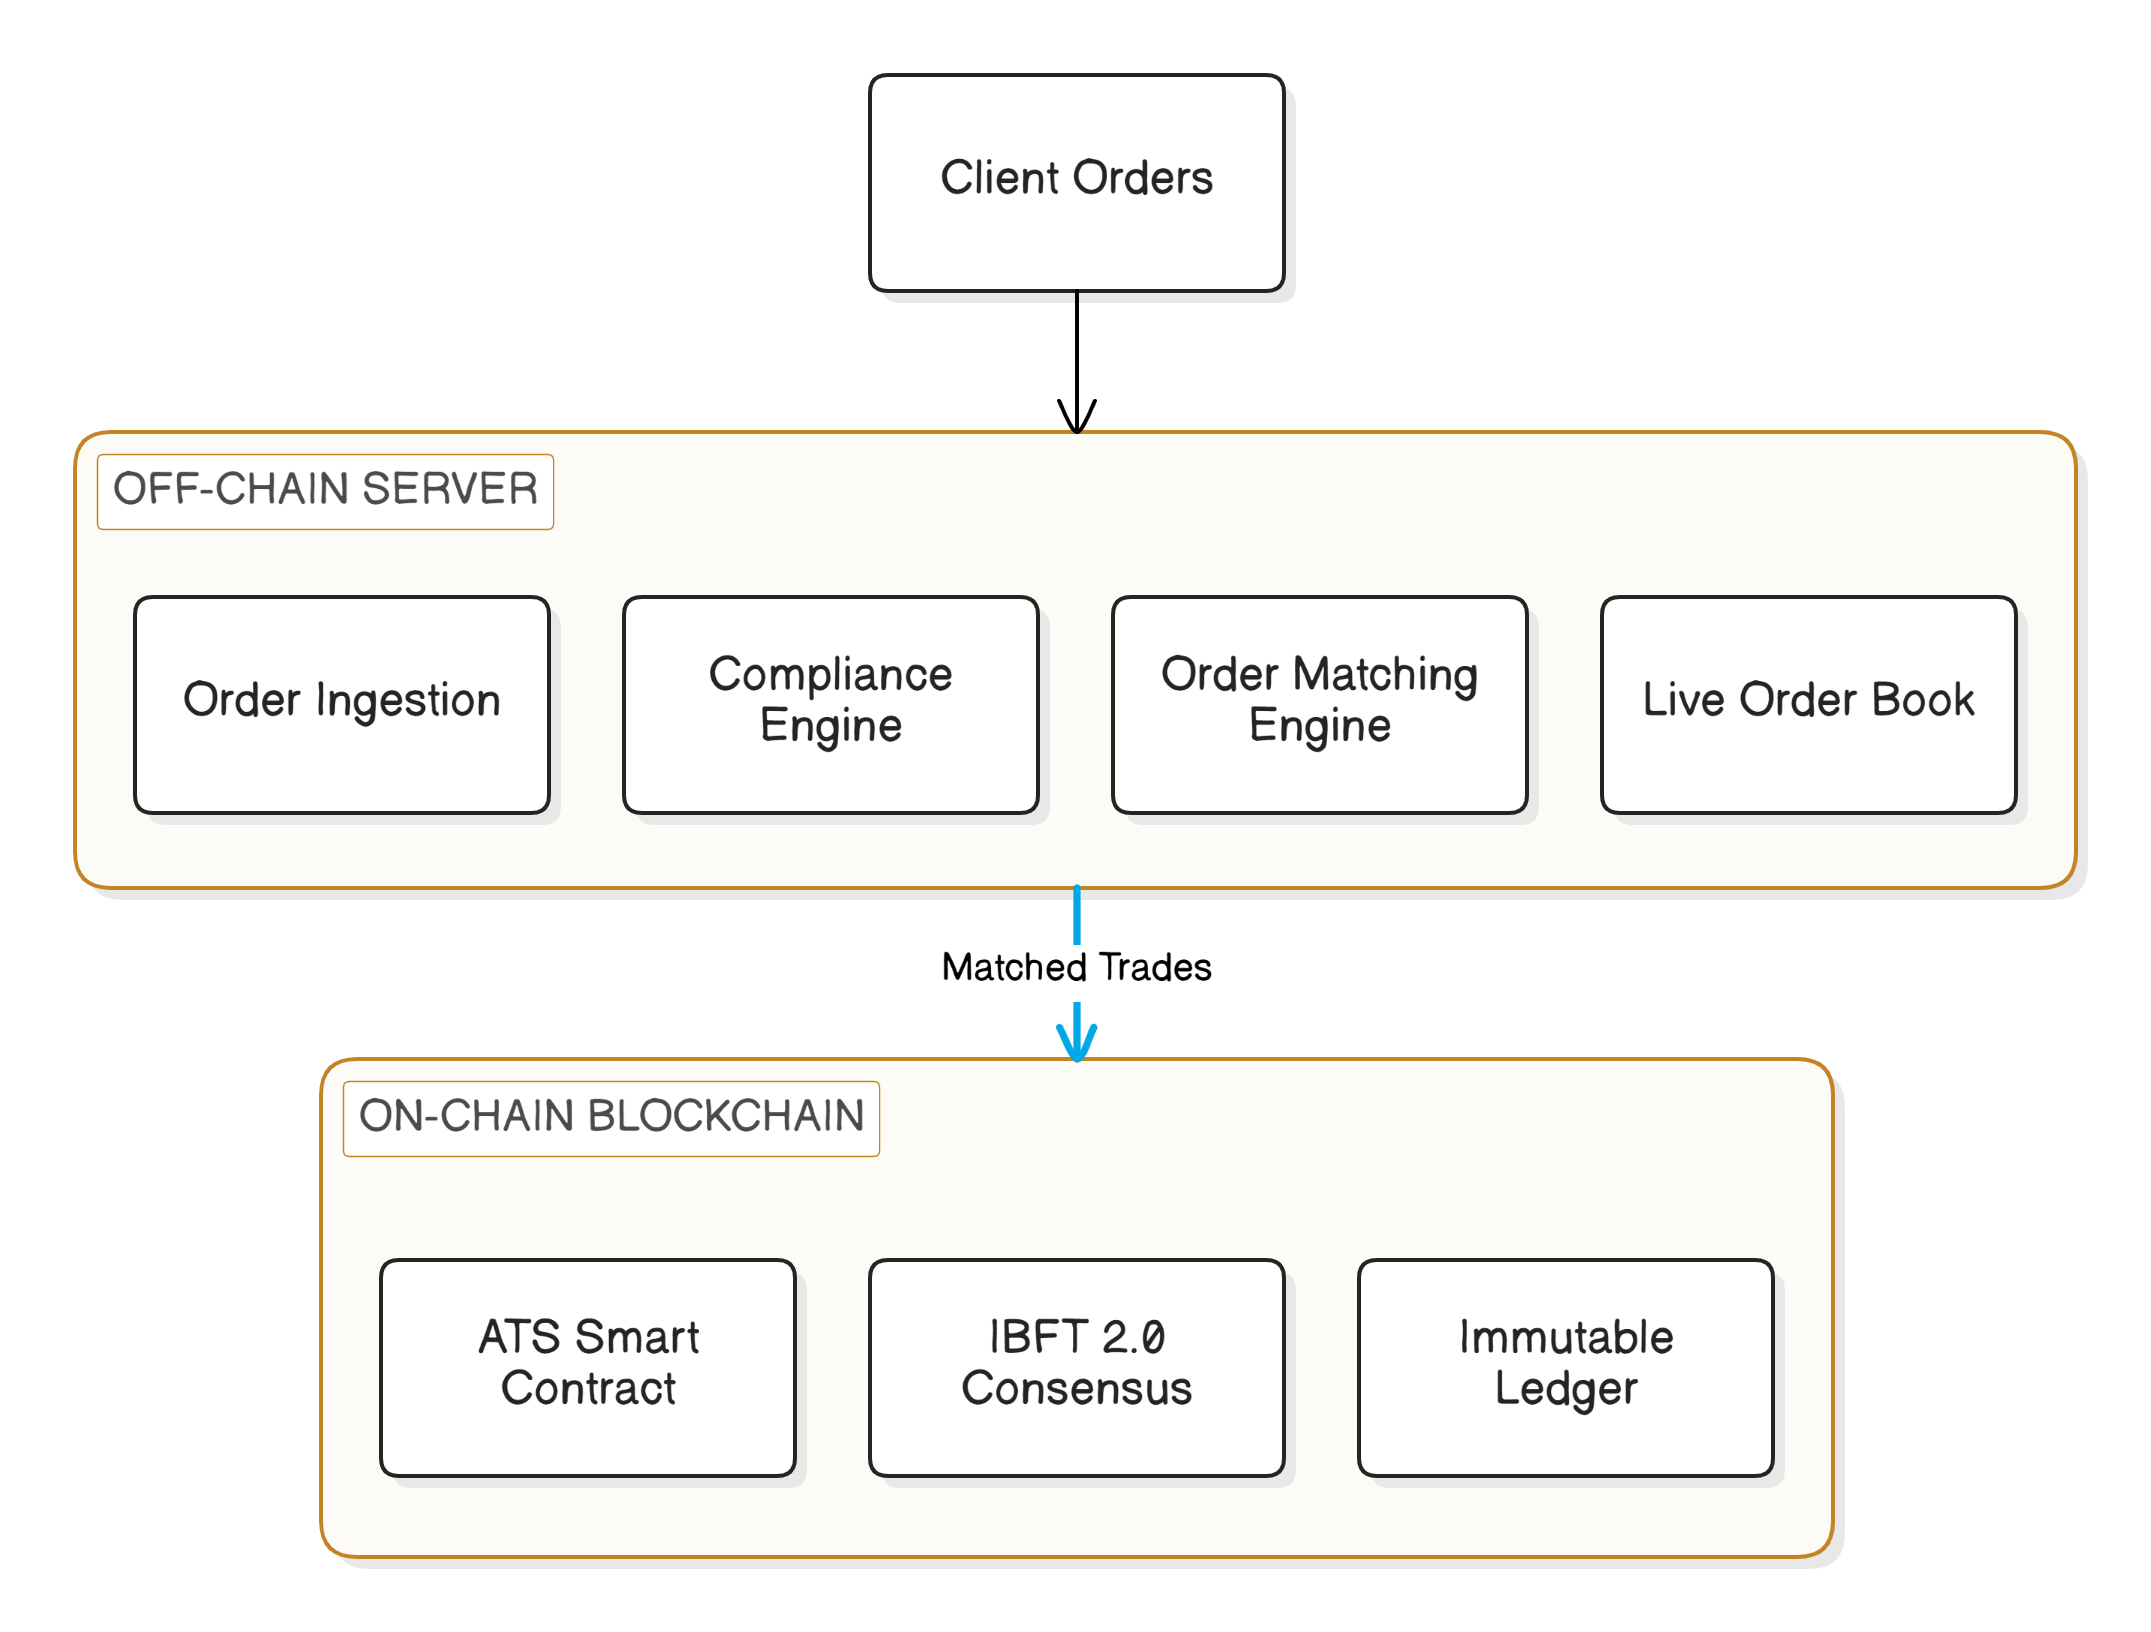
\includegraphics[width=\textwidth]{images/two-layer-model.png}
        \caption{Two-Layer Hybrid Architecture}
        \label{fig:two_layer_model}
    \end{subfigure}
    \hfill
    \begin{subfigure}[b]{0.38\textwidth}
        \centering
        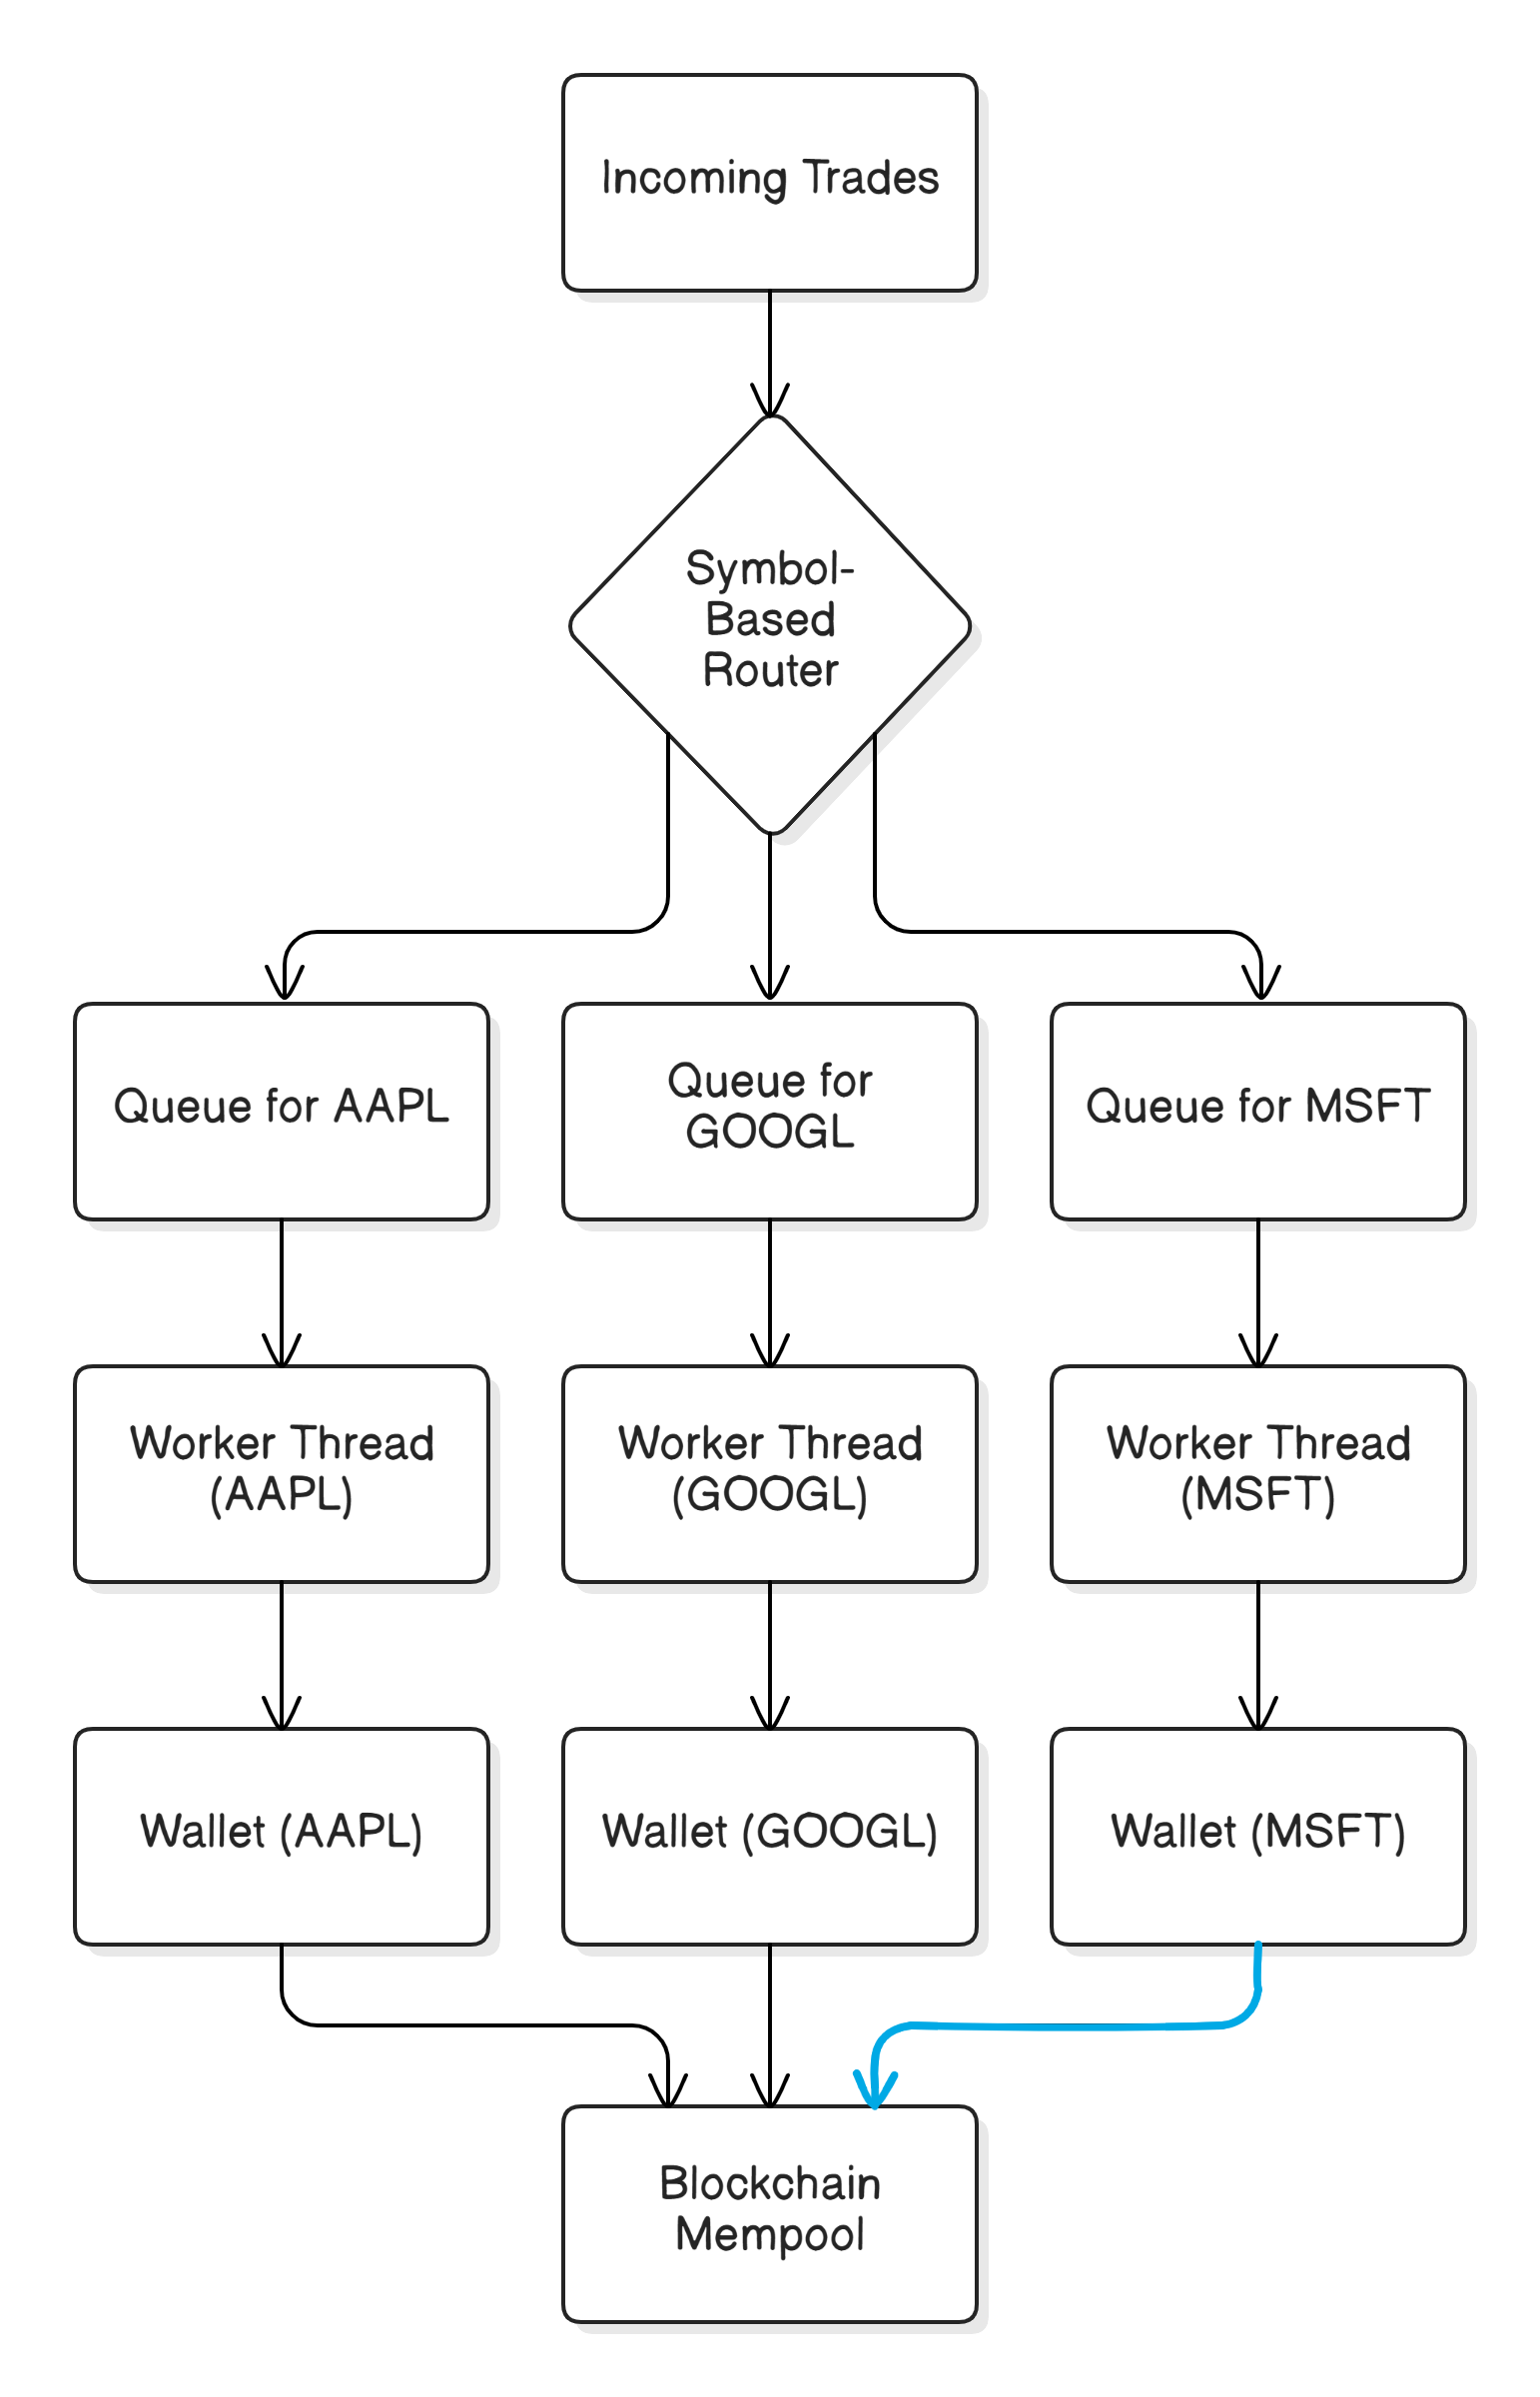
\includegraphics[width=\textwidth]{images/symbol-sharded-lock-free-model.png}
        \caption{Symbol-Sharded Lock-Free Model}
        \label{fig:symbol_sharded_model}
    \end{subfigure}
    \caption{System architecture: (a) Two-layer model separating off-chain compliance from on-chain settlement, (b) Symbol-sharded lock-free model showing end-to-end alignment from symbol queues to dedicated wallets.}
    \label{fig:architecture}
\end{figure}

By combining these two components, we create a system where the unit of parallelism is the trading symbol itself, from the initial ingestion queue to the final on-chain settlement wallet. This holistic approach to sharding is what enables the system to achieve a throughput of 31.19~tx/sec while simultaneously managing server-side latency. Compared to conventional asynchronous multi-threaded architectures (Architecture~3), this represents a \textbf{2.8$\times$ improvement}; the full ablation from a naive synchronous baseline demonstrates a cumulative 125-fold gain. Together, these components constitute \textbf{contribution C1}: a symbol-sharded, lock-free transaction submission model that ensures the submission layer can sustain rates well in excess of the blockchain's gas-based theoretical capacity, guaranteeing it will never become the bottleneck.
